\section{Effect Algorithm}


\begin{frame}{Convolution Overview}

    It is easiest to regard convolution in time as an operation which creates copies of one signal wherever the other has peaks.

    \begin{columns}[t]

        \column{0.3\textwidth}
        \begin{figure}
            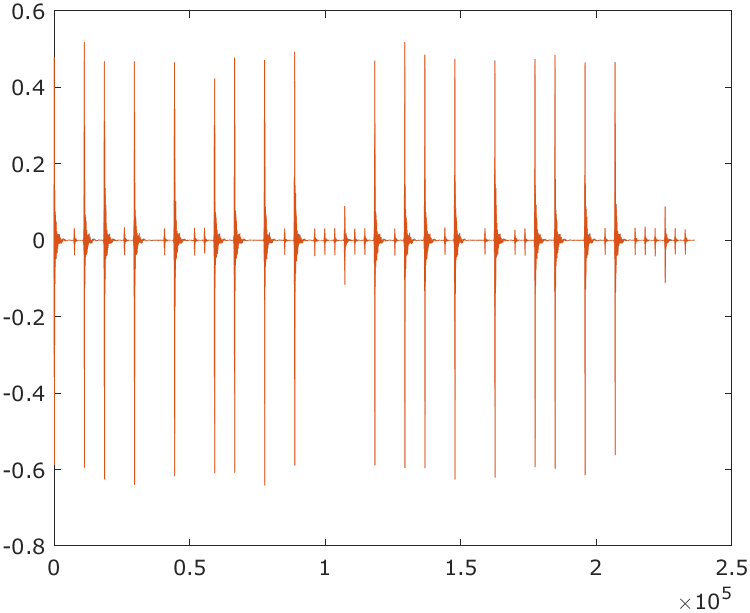
\includegraphics[height=0.4\textheight]{drum-wave}
            \caption{A drum sequence}
        \end{figure}

        \column{0.3\textwidth}
        \begin{figure}
            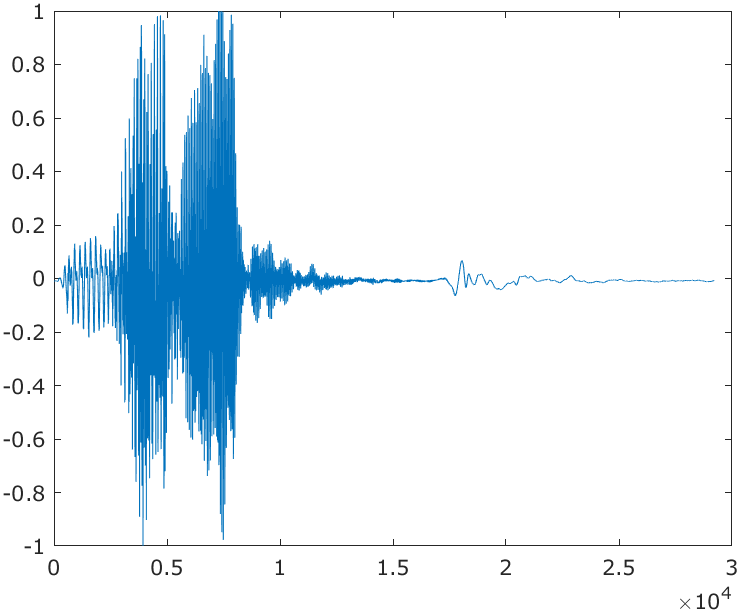
\includegraphics[height=0.4\textheight]{yop-wave}
            \caption{A ``Yop!''}
        \end{figure}

        \column{0.3\textwidth}
        \begin{figure}
            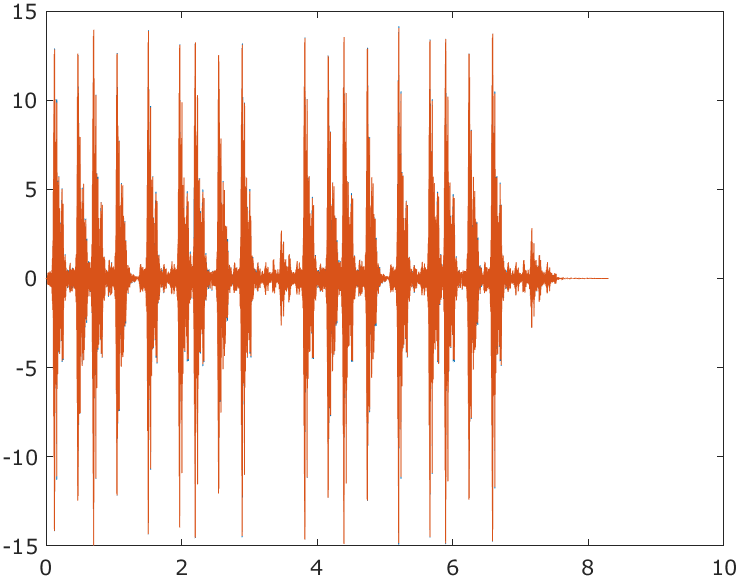
\includegraphics[height=0.4\textheight]{conv-wave}
            \caption{A drum sequence convolved with a ``Yop!''}
        \end{figure}

    \end{columns}

\end{frame}


\begin{frame}{Hardware Challenges}

    Implementing convolution in hardware may be difficult, mostly due to timing constraints.

    \begin{description}
        \item[2048] clock cycles between codec samples
        \item[48000] samples per second
        \item[\textasciitilde{}23.4] samples to process every clock cycle
        \item[\texttimes 2] because stereo
    \end{description}

\end{frame}
